\section{Future Directions}
\label{sec:future}

Our prototype InferSpark system only implements the variational message
passing inference algorithm for certain exponential-conjugate family Bayesian
networks (namely mixtures of Categorical distributions with Dirichlet priors).
In our future work, we plan to include support for other common types of
Bayesian networks (e.g. those with continuous random variables or arbitrary
priors). The VMP algorithm may be no longer applicable to these Bayesian
networks because they may have non-conjugate priors or distributions out of
exponential family. In order to handle wider classes of graphical models, we
also plan to incorporate other inference algorithms (e.g. Belief propagation,
Gibbs Sampling) into our system, which could be quite challenging because we
have to 1) deal with arbitrary models 2) adapt the algorithm to distributed
computing framework.

\begin{figure*}[th]
\centering
    \includegraphics[width=0.8\linewidth]{figs/workflow_future.eps}
    \caption{Future Direction}
    \label{fig:workflow_future}
\end{figure*}

Another interesting future direction is to allow implementation of customized
inference algorithms as plugins to the InferSpark compiler. To make the
development of customized inference algorithms in InferSpark easier than
directly writing them in a distributed computing framework, we plan to further
design a high-level language for implementing algorithms. The resulting
architecture is shown in \figref{fig:workflow_future}. The developers can
implement new algorithms in the high-level language and specifies what models
it supports. InferSpark handles the algorithm matching and translation from
the high-level language into Spark program. This module is similar to efforts
like SystemML, MLI, which targets the algorithm developer but is integrated
into InferSpark. The new modules replaces the hard-coded CodeGen module so the
end-users need to be concerned with the changes.


